\documentclass[10pt,twocolumn,letterpaper]{article}

%% Language and font encodings
\usepackage[english]{babel}
\usepackage[utf8x]{inputenc}
\usepackage[T1]{fontenc}

\usepackage{subcaption}

%% Sets page size and margins
\usepackage[a4paper,top=3cm,bottom=2cm,left=3cm,right=3cm,marginparwidth=1.75cm]{geometry}

%% Useful packages
\usepackage{amsmath}
\usepackage{graphicx}
\usepackage[colorinlistoftodos]{todonotes}
\usepackage[colorlinks=true, allcolors=blue]{hyperref}

\title{Image De-Noising using the $L_0$ Norm}
\author{Josh Kelle}

\begin{document}
\maketitle

\section{Introduction}
This project investigates two statistical methods for removing noise from cartoon images caused by lossy compression. Both methods, $\alpha$-expansion \cite{boykov2001fast} and $L_0$ gradient minimization \cite{xu2011image}, frame this spatial smoothing task as an optimization problem.

The $\alpha$-expansion method models the image as a graph and uses graph cuts to compute a labeling that approximately minimizes graph energy. The $L_0$ gradient minimization method introduces auxiliary variables into the objective function and alternates solving smaller subproblems.

I describe both methods in moderate detail. I then apply both methods to an example cartoon image and compare results.

\section{The Cartoon Domain}
Figure \ref{fig:origcartoon} shows an example image of a cartoon. The image has been compressed and shows the resulting undesired artifacts. Ideally, the girl's bow would be solid pink with just a single pixel value (aside from the black contour). In figure \ref{fig:sadylars} the two characters exiting the building should be composed of clothing and body parts that are each a constant color value. Instead, the compression introduces a lot of noise in this complex scene.

\begin{figure*}
\begin{subfigure}{\textwidth}
  \centering
  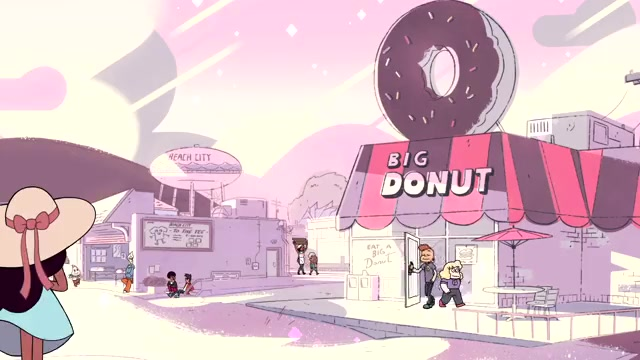
\includegraphics[width=\linewidth]{colorFrame000300.jpg}
  \caption{original noisy image}
  \label{fig:frame300}
\end{subfigure}
\begin{subfigure}{.5\textwidth}
  \centering
  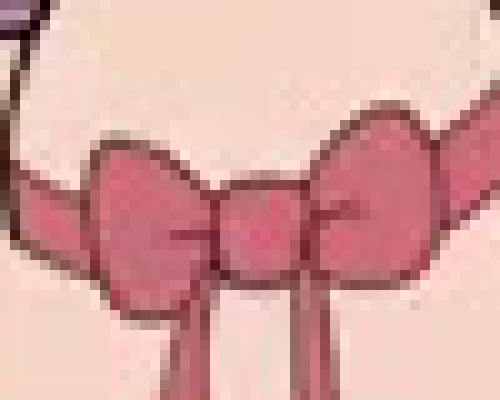
\includegraphics[width=\linewidth]{bow_large.png}
  \caption{cropped and zoomed-in section of the girl's bow}
  \label{fig:bow}
\end{subfigure}
\begin{subfigure}{.5\textwidth}
  \centering
  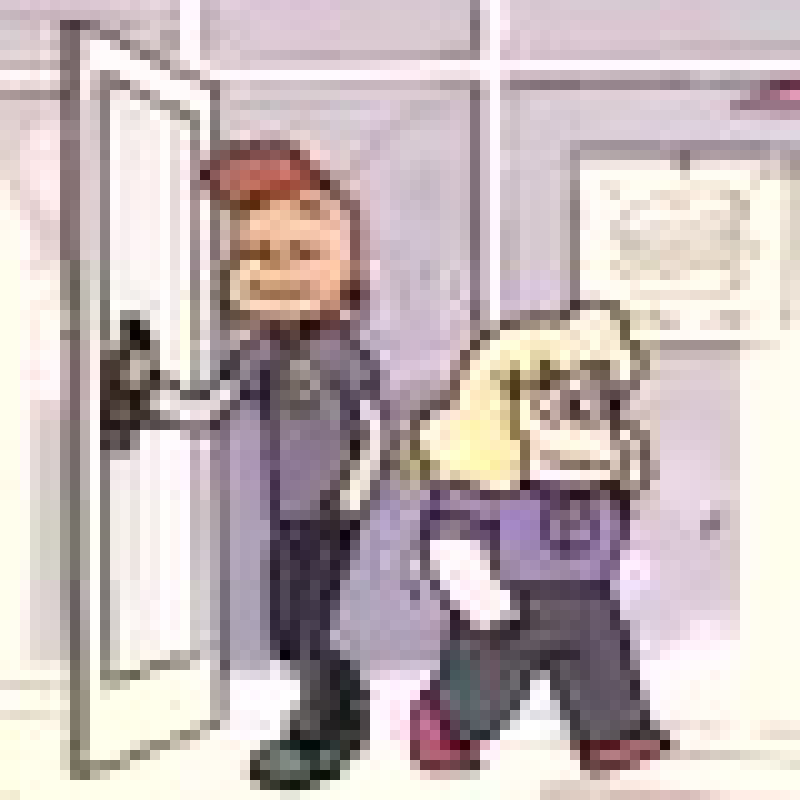
\includegraphics[width=\linewidth]{sady_lars_large.png}
  \caption{cropped and zoomed-in section of characters exiting the donut shop}
  \label{fig:sadylars}
\end{subfigure}
\caption{An example cartoon image. Part \ref{fig:frame300} is the full 640 x 360 resolution image. Parts \ref{fig:bow} and \ref{fig:sadylars} are smaller regions in of the image, zoomed in to make compression artifacts easier to see.}
\label{fig:origcartoon}
\end{figure*}

\section{The Objective Function}

Let $v$ be the raw, noisy image composed of pixels $v_i$. Let $u$ be the smoothed image composed of pixels $u_i$. The objective function $f$ is defined as the sum of two terms.
$$
	f(u, v) = f_{data}(u, v) + f_{smooth}(u)
$$
The $f_{data}$ term measures fit to the data and decreases when $u$ and $v$ are similar. $f_{smooth}$ measures smoothness and decreases when pixels $u_i$ are similar to neighboring pixels $u_j$. The idea is this: if $f_{data}$ and $f_{smooth}$ are well crafted, minimizing $f$ will result in an optimally de-noised image $u$.

\begin{figure}[t]
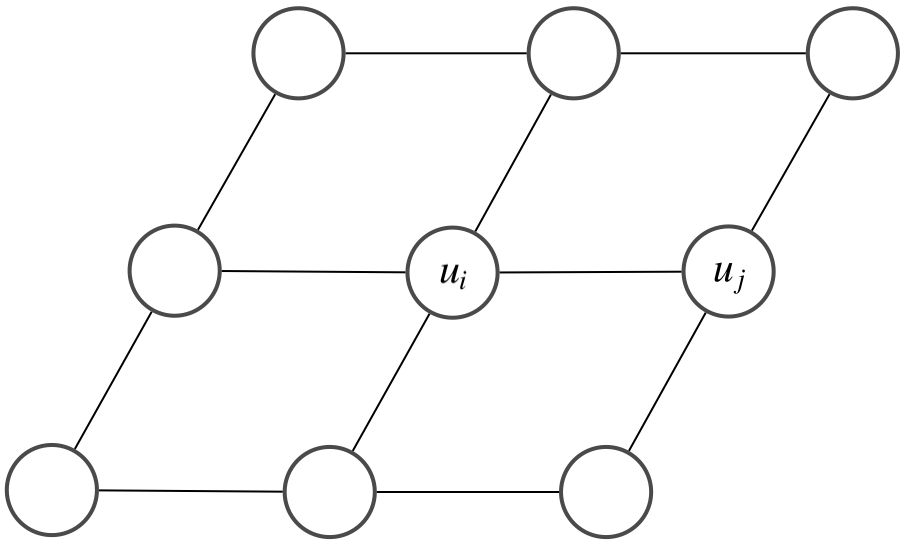
\includegraphics[width = \linewidth]{graph2.png}
\caption{The graphical structure of $G$. Each pixel $u_i$ of the smoothed image is connected to its four neighbors $u_j$.}
\label{fig:graph2}
\end{figure}

\subsection{Choosing $f_{data}$}
If we assume that observed pixels $v_i$ are IID normally distributed with mean $u_i$ and some variance $\sigma^2$, that is $ v_i = u_i + e_i $ where $e_i \sim N(0, \sigma^2) $, then the negative log likelihood yields a quadratic term 
$$
	f_{data}(u, v) = \sum_{i=1}^n{(u_i - v_i)^2} = \left \| u - v \right \|_2^2
$$
Intuitively, this penalizes $u$ more as it deviates from $v$. I use this definition of $f_{data}$ in all experiments.

\subsection{Choosing $f_{smooth}$}

When reasoning about image smoothness, it is often helpful to represent the image as a 4-connected 2D grid graph $G$ where each node $u_i$ represents a pixel. There exists an edge $e_{ij}$ between every adjacent pair of pixels $u_i$ and $u_j$. This graph structure is illustrated in Figure \ref{fig:graph2}.

Many common smoothing functions are a function of $ Du $ where $u$ is the vector representation of the smoothed image and $D$ is the oriented edge matrix. That is, $ D $ is constructed such that $ Du $ gives a vector of the pairwise differences $ u_i - u_j $ for every edge in $ G $. I briefly examine three common definitions of $f_{smooth}$ and compare their usefulness to the task of compression artifact removal of cartoon images.

{\bf Laplacian smoothing: }Laplacian smoothing  measures smoothness by the $L_2$ norm of $Du$.
$$
	f_{smooth} = \lambda \left \| Du \right \|_2^2
$$
Here $\lambda$ is simply a constant hyperparameter that governs the balance between fitting the data and producing a smooth image. Using the $L_2$ norm has the effect of encouraging near-Gaussian smoothness. In this case, optimizing $f$ is approximately equivalent to applying a Gaussian blur convolution to the image. This will ease the appearance of compression artifacts, but it will also diminish sharp edges. In the context of cartoons, the true image usually consists of several regions of constant color with sharp color differences at their boundaries. Therefore, Laplacian smoothing is not a good choice for this domain.

{\bf Graph-Fused LASSO: } Graph-fused LASSO (GFL) measures smoothness by the $L_1$ norm of $Du$.
$$
	f_{smooth} = \lambda \left \| Du \right \|_1
$$
In contrast to Laplacian smoothing, using the $L_1$ norm has the effect of encouraging regions of constant color while maintaining sharper changes between regions. However, adjacent regions are still encouraged to be similar in color. For the cartoon dataset, GFL will ease the appearance of compression artifacts, but adjacent regions need not be similar in color. In fact they usually aren't, as shown in Figure \ref{fig:origcartoon}. Furthermore, using the $L_1$ also causes the regions' color value of to "shrink" towards the mean color, another undesirable property.

{\bf Potts Model: } The Potts Model defines the smoothness function as follows
$$
	f_{smooth} = \lambda \min(1, |u_i - u_j|) = \lambda \left \| Du \right \|_0
$$
Since pixels $u_i$ are integers, this is equivalent to counting the number adjacent pixels that differ in color. This definition is equivalent to the $L_0$ norm of $Du$. Similar to the GLF, this model encourages regions of constant color. In contrast to the GFL, adjacent color regions incur the same penalty regardless of how similar or different they are in color. This is an appropriate property for the cartoon domain. I use this definition of $f_{smooth}$ in all experiments.

Putting this all together, we have the following objective function:
\begin{align} \label{eq:objfn0}
	f(u, v) &= f_{data}(u, v) + f_{smooth}(u) \\
    &= \left \| u - v \right \|_2^2 + \lambda \left \| Du \right \|_0 \label{eq:objfn}
\end{align}


\section{The $\alpha$-Expansion Method}
The $\alpha$-expansion method published by Boykov et al. (2001) models the image as a graph and uses a series of graph cuts to approximately minimize the energy of the graph \cite{boykov2001fast}. In this section, I define the graph, its energy function, graph cuts on a binary image, and finally the full $\alpha$-expansion algorithm.

{\bf Graph: } Define a graph $G’$ to be an augmented version of $G$. The vertex set contains nodes $u_i$ that represent pixels in the smoothed image and nodes $v_i$ that represent corresponding pixels in the noisy raw image. Like in $G$, there exists an edge $e_{ij}$ between every adjacent pair of nodes $u_i$ and $u_j$. Additionally, there exists an edge $e_i$ between every pair of nodes $u_i$ and $v_i$. Figure \ref{fig:graph} illustrates the graph structure.

\begin{figure}[t]
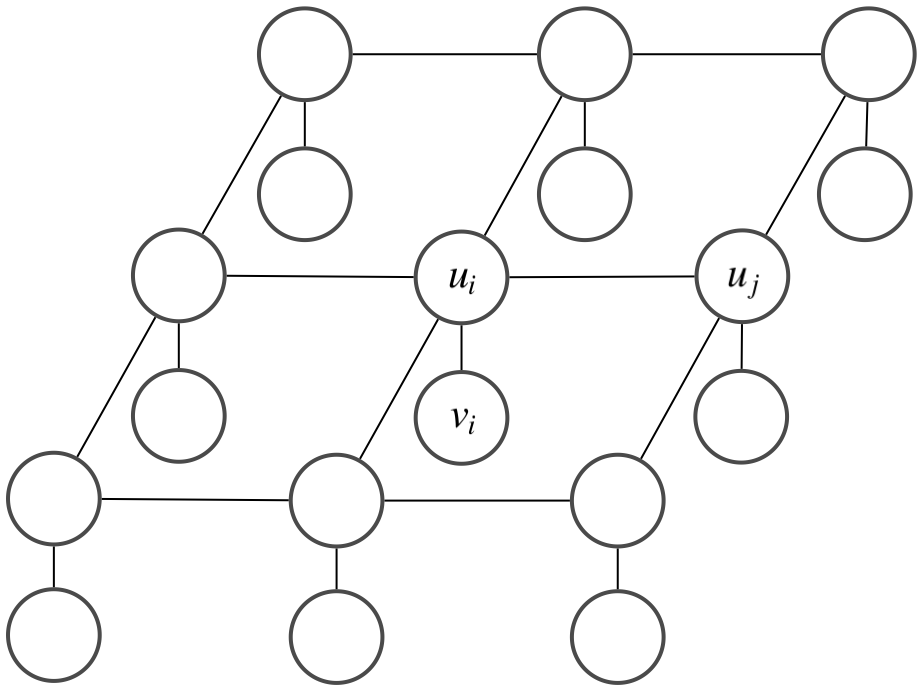
\includegraphics[width = \linewidth]{graph.png}
\caption{The graphical structure of $G'$. Each pixel $u_i$ of the smoothed image is connected to its four neighbors $u_j$ in the smoothed image and its corresponding pixel $v_i$ in the raw image.}
\label{fig:graph}
\end{figure}

{\bf Energy function: }	The energy function $E:G’ \rightarrow {\rm I\!R} $ is mathematically identical to the objective function $f$ defined in the previous section.
\begin{align*}
	E(u, v) &= E_{data}(u, v) + E_{smooth}(u) \\
    &= \left \| u - v \right \|_2^2 + \lambda \left \| Du \right \|_0
\end{align*}

Aside: In context of graphs, it is convention to refer to the objective function as an "energy function." Minimizing energy to reach an optimal state is an analogy borrowed from physics.

{\bf Graph cuts: } Consider the case of a binary image - an image with only two colors. The image is modeled by the graph $G'$ but with two extra  nodes $s$ and $t$. For every node $u_i$ there are two new edges, one to $s$ and one to $t$. The nodes $s$ and $t$ do not correspond to pixels in the image, but instead correspond to the two colors, or \textit{labels}. An $st$-cut on the graph is defined as a minimal set of edges $e_{ij}$ such that removing these edges partitions the graph into two connected components, one connected to $s$ and the other to $t$. That is, once these edges are removed, there is no longer a path from $s$ to $t$. Nodes $u_i$ with a path to $t$ are labeled with color $t$, and vise versa for those with a path to $s$. A min-cut is the $st$-cut whose sum of edge weights is minimum. A min-cut corresponds to a labeling $u$ that minimizes the energy, and is thus the optimally de-noised image.

{\bf $\alpha$-expansion: } The special case of binary labeling can be solved exactly in polynomial time, but the general case of multiple labels remains NP-hard. The $\alpha$-expansion algorithm approximates the exact solution by applying a series of binary graph cuts, each of which takes a local greedy move toward minimizing the energy. A single expansion move is as follows: for a given label $\alpha$, let any pixels whose current label is not $\alpha$ either switch to $\alpha$ or remain the same. Given a label $\alpha$, construct a new graph such that the min-cut labeling minimizes energy.

The $\alpha$-expansion algorithm iteratively cycles through all labels, applying the single expansion moves until energy stops decreasing. It is important to note that $\alpha$-expansion is guaranteed to decrease energy only if the $E_{smooth}$ is a metric, meaning it satisfies these three properties:
\begin{enumerate}
    \item $g(\alpha, \beta) = 0 \leftrightarrow \alpha = \beta$, or
    $\\ g(\alpha, \beta) \neq 0 \leftrightarrow \alpha \neq \beta$
  \item $g(\alpha, \beta) = g(\beta, \alpha) \geq 0$
    \item $g(\alpha, \beta) \leq g(\alpha, \gamma) + g(\gamma, \beta)$
\end{enumerate}

\section{The $L_0$ Gradient Minimization Method}
Xu et al. (2011) describe a different method for approximately minimizing equation \ref{eq:objfn} in their paper Image Smoothing via $L_0$ Gradient Minimization \cite{xu2011image}. Instead of modeling the image as a graph and computing graph cuts, the authors augment the objective function with auxiliary variables and propose an alternating minimization solver that iteratively updates different sets of variables until convergence. This method has the same effect of suppressing low-amplitude image structures while preserving salient edges. In addition to compression artifact removal in cartoons, the authors also claim their method is useful for edge extraction, non-photorealistic effect generation, and detail enhancement.

The authors formulate the objective function as
\begin{equation} \label{eq:objfn2}
\min_S \left\lbrace \sum_p(S_p - I_p)^2 + \lambda C(S) \right\rbrace
\end{equation}
where $I$ is the noisy image, $S$ is the smoothed image, $p$ indexes pixels, $\lambda$ is the smoothness hyperparameter as defined before, and $C(S) = \#\left\lbrace p \mid |\partial_xS_p| + |\partial_yS_p| \neq 0 \right\rbrace$ counts the number of times a pixel $S_p$ differs from its neighbors. It is easy to see that equation \ref{eq:objfn2} is mathematically equivalent to equation \ref{eq:objfn}.

The authors approximately solve this optimization problem by introducing auxiliary variables $h_p$ and $v_p$ into the objective function to create a new augmented objective

\begin{align*}
\min_{S,h,v} \Biggl\lbrace &\sum_p(S_p - I_p)^2 + \lambda C(h, v) \Biggr.\\
+ \Biggl. &\sum_p\beta((\partial_xS_p - h_p)^2 + (\partial_yS_p - v_p)^2) \Biggr\rbrace
\end{align*}
where $C(h, v) = \#\left\lbrace p \mid |h_p| + |v_p| \neq 0 \right\rbrace$ and $\beta$ is an automatically adapting parameter that controls the similarity between $(h, v)$ and their respective gradients. Notice that this equation approaches equation \ref{eq:objfn2} as $\beta$ becomes large. The variables $h_p$ and $v_p$ correspond to $\partial_xS_p$ and $\partial_yS_p$ respectively ($h$ for "horizontal" and $v$ for "vertical").

Each iteration of the solver solves two subproblems. The first subproblem updates $S$ while keeping $h$ and $v$ fixed. The second subproblem updates $h$ and $v$ while keeping $S$ fixed.

{\bf Updating $S$: } Omitting terms that don't involve $S$ gives the following quadratic optimization subproblem, which can be solved by gradient descent.

\begin{align*}
\min_{S} \Biggl\lbrace &\sum_p(S_p - I_p)^2 \Biggr.\\
+ \Biggl. &\sum_p\beta((\partial_xS_p - h_p)^2 + (\partial_yS_p - v_p)^2) \Biggr\rbrace
\end{align*}
The authors describe an alternative, faster method of solving this subproblem using the Fast Fourier Transform, but I won't cover it here.

{\bf Updating $(h, v)$: } Omitting terms that don't involve $h$ or $v$ gives the following optimization problem.
\begin{align*}
\min_{h,v} \Biggl\lbrace & \frac{\lambda}{\beta} C(h, v) \Biggl. \\ 
& \Biggl. + \sum_p((\partial_xS_p - h_p)^2 + (\partial_yS_p - v_p)^2) \Biggr\rbrace
\end{align*}
The key here is this expression can be decomposed such that each $h_p$ and $v_p$ are estimated individually, which gives the following:
\begin{align*}
\sum_p \min_{h_p,v_p} \Biggl\lbrace & \frac{\lambda}{\beta} H(|h_p| + |v_p|) \Biggr. \\
& + \Biggl. (\partial_xS_p - h_p)^2 + (\partial_yS_p - v_p)^2 \Biggr\rbrace
\end{align*}
where $H(|h_p| + |v_p|)$ is a binary indicator function that returns 1 if $|h_p| + |v_p| = 0$ and 0 otherwise. Each term in the summation reaches a minimum under the condition
\[ 
(h_p, v_p) =
\begin{cases} 
      (0, 0) & (\partial_xS_p)^2 + (\partial_yS_p)^2 < \lambda/\beta \\
      (\partial_xS_p, \partial_yS_p) & \text{otherwise} \\
   \end{cases}
\]
The authors provide a proof of this claim in their paper, but I won't repeat it here.

\section{Experiments}
In this section I apply both methods to the cartoon shown in figure \ref{fig:origcartoon}. In both cases, I use code provided from the respective authors.

\subsection{Smoothing with $\alpha$-expansion}
Let $n$ be the number of pixels in the image, and let $\mathcal{L} = \left\lbrace l_1, l_2, ..., l_m \right\rbrace $ be the set of allowable labels/colors. In the provided C\texttt{++} code \cite{boykov2001fast, kolmogorov2004energy, boykov2004experimental}, the user defines $f_{data}(u_i, v_i)$ as a matrix $A \in {\rm I\!R}^{n \times m}$ where $A_{i,j}$ contains the cost incurred from labeling pixel $u_i$ with color $l_j$. The user defines $f_{smooth}(u_i, u_j)$ as a matrix $B \in {\rm I\!R}^{m \times m}$ where $B_{i, j}$ contains the cost incurred from labeling some pixel with color $l_i$ when one of its neighboring pixels is labeled with color $l_j$. These two matrices are provided to the solver and fully define the problem.

Note the flexibility of this setup. It allows for any custom definition of $f_{data}$ and $f_{smooth}$, not just those given by equation \ref{eq:objfn}. However, I define the matrices according to equation \ref{eq:objfn} unless otherwise specified.

Applying $\alpha$-expansion to a grayscale image is straightforward. But how can one apply this method to a color image? I explore 3 options here.

{\bf Option 1: Independent channels } One option is to treat each of the three color channels separately by running three instances of $\alpha$-expansion to get three smoothed images, and then merge the results. However, these three color channel images might result in a different segmentation, in which case it is unclear to me how to merge them into a single smoothed color image.

{\bf Option 2: Color encoding } Another option is to map a color $c = (c_1, c_2, c_3) \in {\rm I\!R}^3$ to a scalar $c' \in {\rm I\!R}$. Since each color channel has the range $[0, 255]$, I construct the following mapping that simply concatenates the 8 bits of each color channel: $c' = (c_1 \ll 16) \lor (c_2 \ll 8) \lor c_3$ where "$\ll$" is the bit-wise left shifting operator and "$\lor$" is the bit-wise OR operator. Given $c'$, one can recover the three separate channels by similar bit-wise logic.

With this mapping, the size of the label space $\mathcal{L}$ is $m = 256^3 = 16,777,216$. The image in figure \ref{fig:frame300} has dimension $640 \times 360$. This means the data cost matrix $A$ would have dimension $n \times m = 230,400 \times 16,777,216$ which is more than 3.8 trillion entries. This is intractable.

Instead of using all possible $256^3$ labels, what if we used just the labels present in the original image? The worst case occurs when every pixel in the image is a different color. This leads to $m = n = 640*360 = 230,400$. Then $A$ would have $n^2 = 230,400^2 \approx 53$ billion entries. Assuming each element takes 32 bits of memory, this results in a matrix of size about 200 GB. This is still intractable.

But that's worst case. The image in figure \ref{fig:frame300} actually has only 39,725 distinct colors. This would result in a matrix $A$ with $m \times n = 39,725 * 230,400 \approx 9$ billion entries, which would require about 34 GB of memory. Still intractable for my laptop.

Luckily, the authors'  code has an alternative to instantiating these large matrices. Instead, one can define C++ functions that compute these costs on the fly, as needed. (If memory is not a concern, this option will probably slower than using the matrices.) I try this option, but the algorithm still needs to cycle through all $m$ labels, and in my experience each iteration can take several minutes. So it is still very slow.

{\bf Option 3: Grayscale transfer } One option is to convert the color image to grayscale, invoke $\alpha$-expansion to segment the image into color-constant regions, convert back to a color image, and paint these regions with the their respective average color in the original image. By "paint" I mean to overwrite pixel values. In this scenario, there are only $m = 256$ labels. This results in the data cost matrix $A$ having $256 * 230,400 \approx 60$ million, which requires about 225 MB of memory. This is tractable! The smoothness cost matrix $B$ will have $256^2 = 65,536$ entries which turns out to require 256 KB of memory. Not much at all compared to $A$.

Therefore, I chose to pursue option 3, grayscale transfer. Results across different values of lambda are shown in figure \ref{fig:alphaResultsFull}. For smaller values of $\lambda$, you can see how the sky gets merged into fewer regions. As $\lambda$ gets larger, the image becomes smoother. For $\lambda = 1600$, the image is over-smoothed. Much of the salient detail has been erased. Figure \ref{fig:alphaPlot} shows how the number of regions varies as a function of $\lambda$. Here, "number of regions" is a proxy for smoothness - fewer regions implies more smooth. Figures \ref{fig:alphaResultsBow} and \ref{fig:alphaResultsSadylars} shows results for the zoomed-in sections of the girls bow and the characters exiting the donut shop.

\begin{figure}
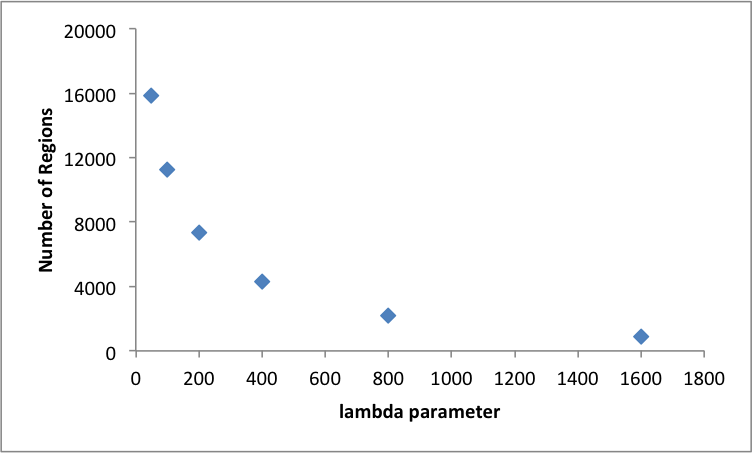
\includegraphics[width=\linewidth]{alphaResults/alphaResultGraph.png}
\caption{This plot shows how the number of regions decreases as $\lambda$ increases. In other words, the image gets segmented into fewer colors, becoming smoother.}
\label{fig:alphaPlot}
\end{figure}

\subsection{Smoothing with $L_0$ gradient minimization}
The authors of \cite{xu2011image} provide MATLAB code that implements their solver. It handles color images out of the box, so using it is more straightforward than using the provided $\alpha$-expansion code. I did, however, slightly modify the MATLAB code - I increased the parameter $\beta_{max}$ which increases accuracy at the cost of longer execution time. Results for different values of $\lambda$ are shown in figures \ref{fig:gradminResultsFull} - \ref{fig:gradminResultsSadylars}.

Notice how the results from this method also become more smooth as $\lambda$ increases. However, the results aren't the same as those from $\alpha$-expansion. The segmentation and smoothing style is different between the two methods despite having mathematically equivalent objective functions. This is because neither method solves the optimization problem exactly. Both methods are approximations, and can thus lead to different results.

\section{Comparing methods}
It is clear that both methods can be used to remove compression artifacts in images. So which method should be used? This section briefly reviews the tradeoffs between the two methods.

{\bf Style: } Figures \ref{fig:alphaResultsFull} and \ref{fig:gradminResultsFull} show that the two methods produce different high-level styles when enough smoothing happens (when $\lambda$ is large). Results from $L_0$ gradient minimization produce smoother, blurrier large structures. An example of this is the sky in these figures.

{\bf Time vs flexibility: } In my experience, $L_0$ gradient minimization is several times faster than $\alpha$-expansion. Part of the reason is that the $L_0$ gradient minimization method always assumes the objective function to be defined as in equation \ref{eq:objfn}. The solver leverages this fact to produce a faster algorithm. On the other hand, with $\alpha$-expansion the practitioner is free to define any arbitrary data cost function $f_{data}$ and smoothness cost function $f_{smooth}$ they want (as long as $f_{smooth}$ satisfies the three metric properties). This is powerful and appealing to anyone who wants to experiment with smoothness cost functions. The price paid for this flexibility is longer computation time.

In short, neither method is superior in all cases. The right method to use depends on the goals and constraints of the project.

\section{Conclusion}
I investigated two methods for removing lossy compression artifacts from cartoon images. Both methods aim to achieve this goal by minimizing the objective function defined by equation \ref{eq:objfn}. However, minimizing this objective exactly is NP-hard, so both methods compute an approximation.
One method, $\alpha$-expansion, models the image as a graph and computes a low-energy labeling via graph cuts. The other method, $L_0$ gradient minimization, augments the the objective function with auxiliary variables and alternates solving for one set of variables while keeping the rest fixed. I showed that both methods can successfully smooth out compression artifacts, though doing so without over smoothing requires careful tuning of the $\lambda$ parameter.



\begin{figure*}
\centering
\begin{subfigure}{.48\linewidth}
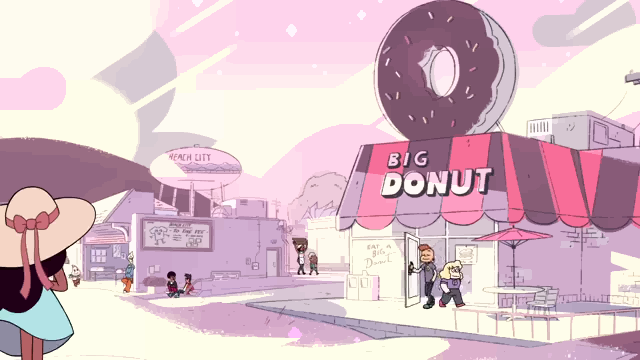
\includegraphics[width=\linewidth]{alphaResults/transfered_050_001_13.png}
\caption{$\lambda = 50$}\label{fig:mouse}
\end{subfigure}
\begin{subfigure}{.48\linewidth}
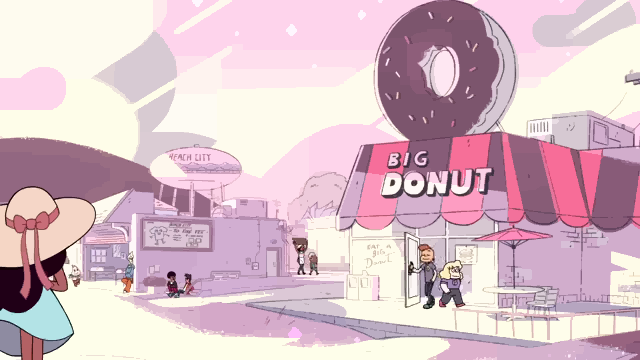
\includegraphics[width=\linewidth]{alphaResults/transfered_100_001_13.png}
\caption{$\lambda = 100$}\label{fig:transfer100}
\end{subfigure}
\begin{subfigure}{.48\linewidth}
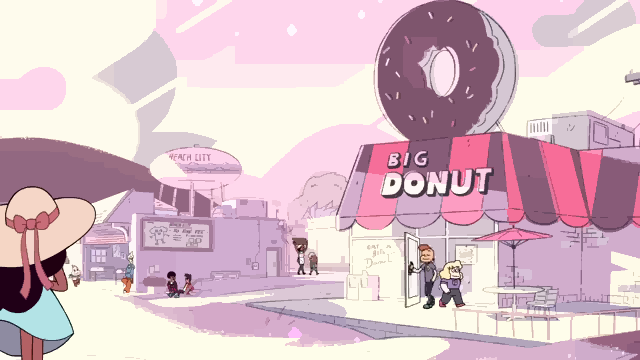
\includegraphics[width=\linewidth]{alphaResults/transfered_200_001_10.png}
\caption{$\lambda = 200$}\label{fig:transfer200}
\end{subfigure}
\begin{subfigure}{.48\linewidth}
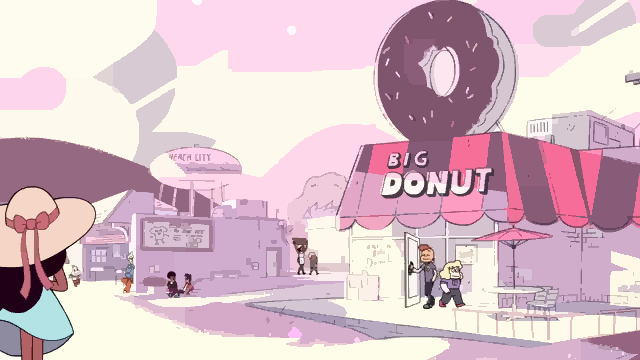
\includegraphics[width=\linewidth]{alphaResults/transfered_400_001_09.png}
\caption{$\lambda = 400$}\label{fig:transfer400}
\end{subfigure}
\begin{subfigure}{.48\linewidth}
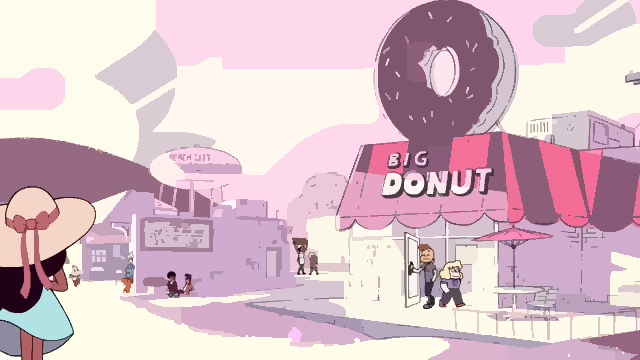
\includegraphics[width=\linewidth]{alphaResults/transfered_800_001_11.png}
\caption{$\lambda = 800$}\label{fig:transfer800}
\end{subfigure}
\begin{subfigure}{.48\linewidth}
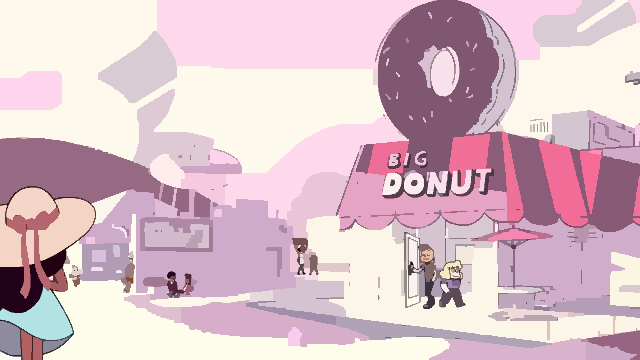
\includegraphics[width=\linewidth]{alphaResults/transfered_1600_001_10.png}
\caption{$\lambda = 1600$}\label{fig:transfer1600}
\end{subfigure}
\caption{Results of $\alpha$-expansion over different values of $\lambda$. These results were generated by the grayscale transfer method.}
\label{fig:alphaResultsFull}
\end{figure*}

\begin{figure*}
\centering
\begin{subfigure}{.48\linewidth}
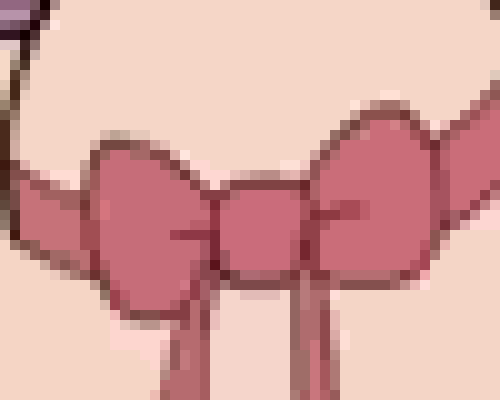
\includegraphics[width=\linewidth]{alphaResults/bow_large_0050.png}
\caption{$\lambda = 50$}
\end{subfigure}
\begin{subfigure}{.48\linewidth}
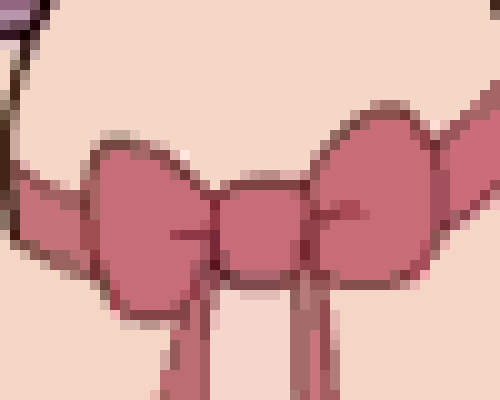
\includegraphics[width=\linewidth]{alphaResults/bow_large_0100.png}
\caption{$\lambda = 100$}
\end{subfigure}
\begin{subfigure}{.48\linewidth}
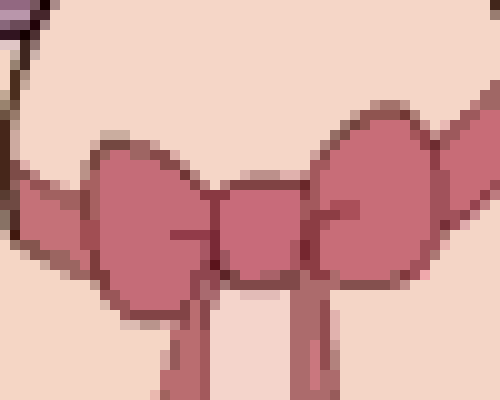
\includegraphics[width=\linewidth]{alphaResults/bow_large_0200.png}
\caption{$\lambda = 200$}
\end{subfigure}
\begin{subfigure}{.48\linewidth}
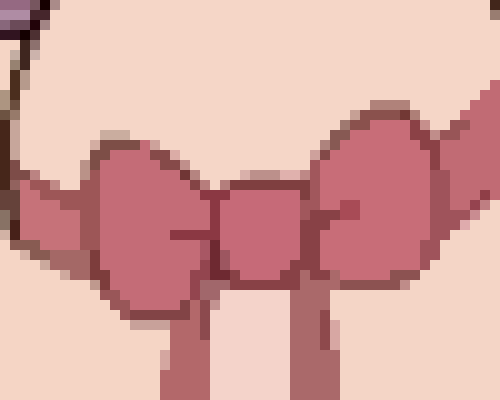
\includegraphics[width=\linewidth]{alphaResults/bow_large_0400.png}
\caption{$\lambda = 400$}
\end{subfigure}
\begin{subfigure}{.48\linewidth}
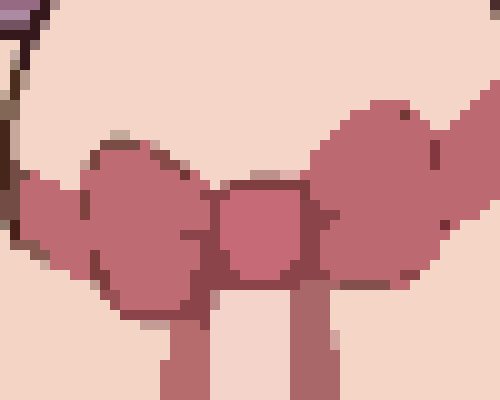
\includegraphics[width=\linewidth]{alphaResults/bow_large_0800.png}
\caption{$\lambda = 800$}
\end{subfigure}
\begin{subfigure}{.48\linewidth}
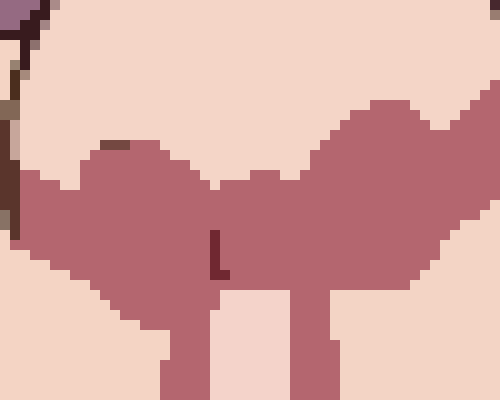
\includegraphics[width=\linewidth]{alphaResults/bow_large_1600.png}
\caption{$\lambda = 1600$}
\end{subfigure}
\caption{Results of $\alpha$-expansion over different values of $\lambda$, zoomed in to see results more easily. These results were generated by the grayscale transfer method.}
\label{fig:alphaResultsBow}
\end{figure*}

\begin{figure*}
\centering
\begin{subfigure}{.48\linewidth}
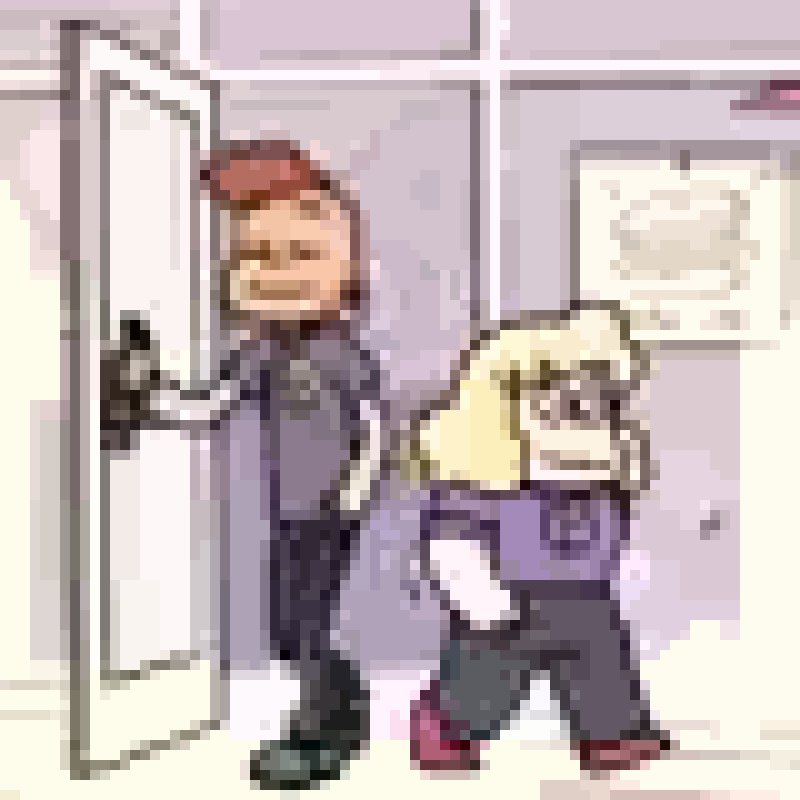
\includegraphics[width=\linewidth]{alphaResults/sadylars_large_0050.png}
\caption{$\lambda = 50$}
\end{subfigure}
\begin{subfigure}{.48\linewidth}
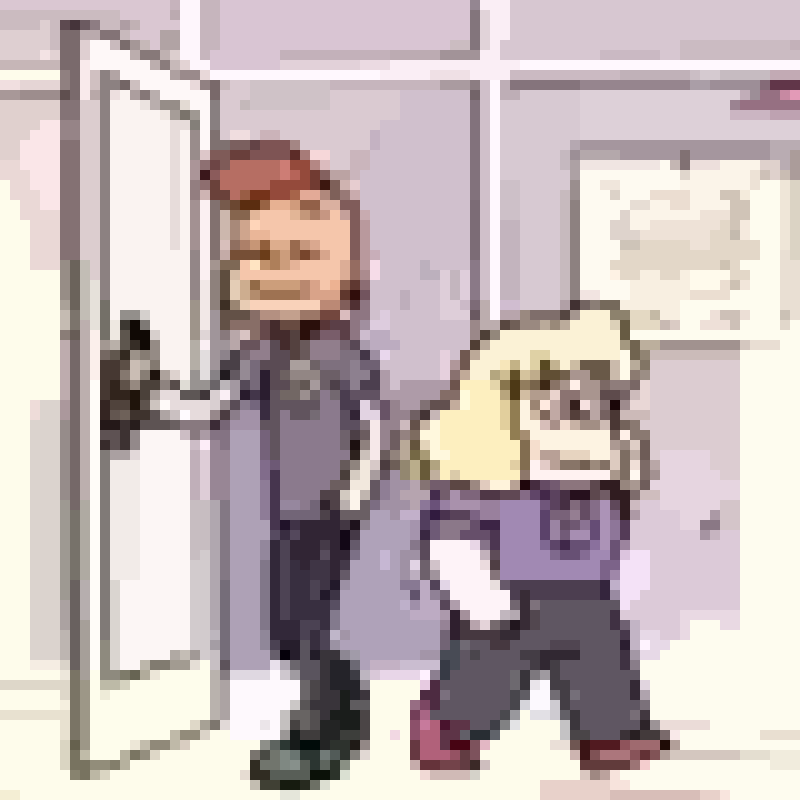
\includegraphics[width=\linewidth]{alphaResults/sadylars_large_0100.png}
\caption{$\lambda = 100$}
\end{subfigure}
\begin{subfigure}{.48\linewidth}
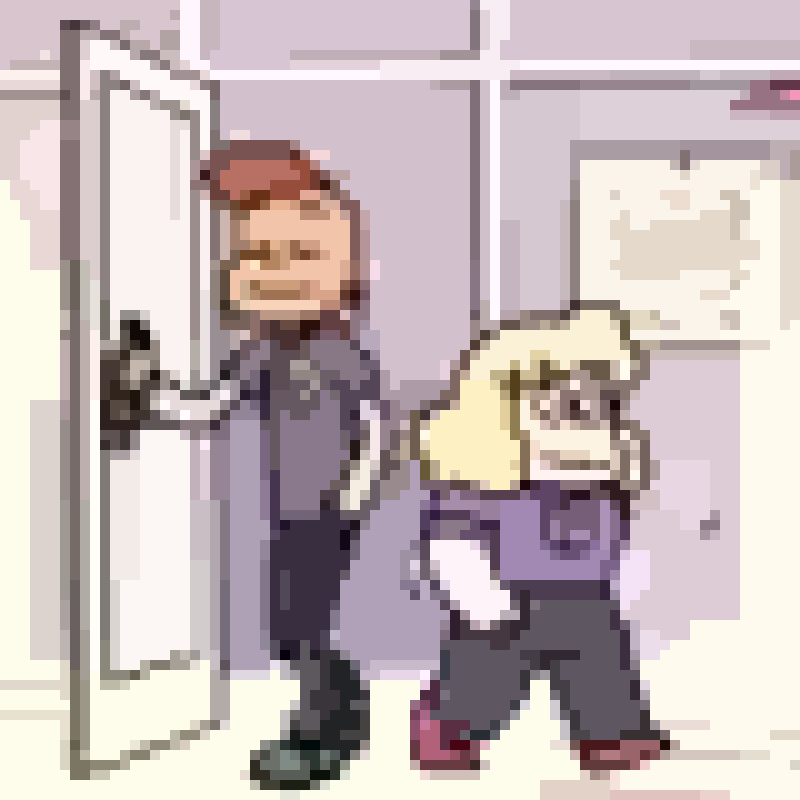
\includegraphics[width=\linewidth]{alphaResults/sadylars_large_0200.png}
\caption{$\lambda = 200$}
\end{subfigure}
\begin{subfigure}{.48\linewidth}
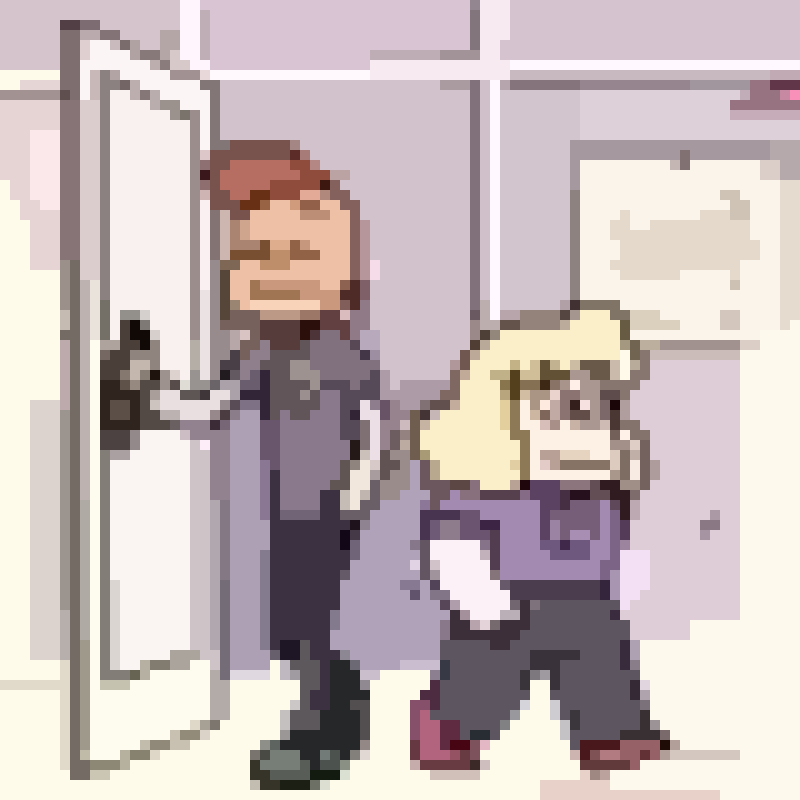
\includegraphics[width=\linewidth]{alphaResults/sadylars_large_0400.png}
\caption{$\lambda = 400$}
\end{subfigure}
\begin{subfigure}{.48\linewidth}
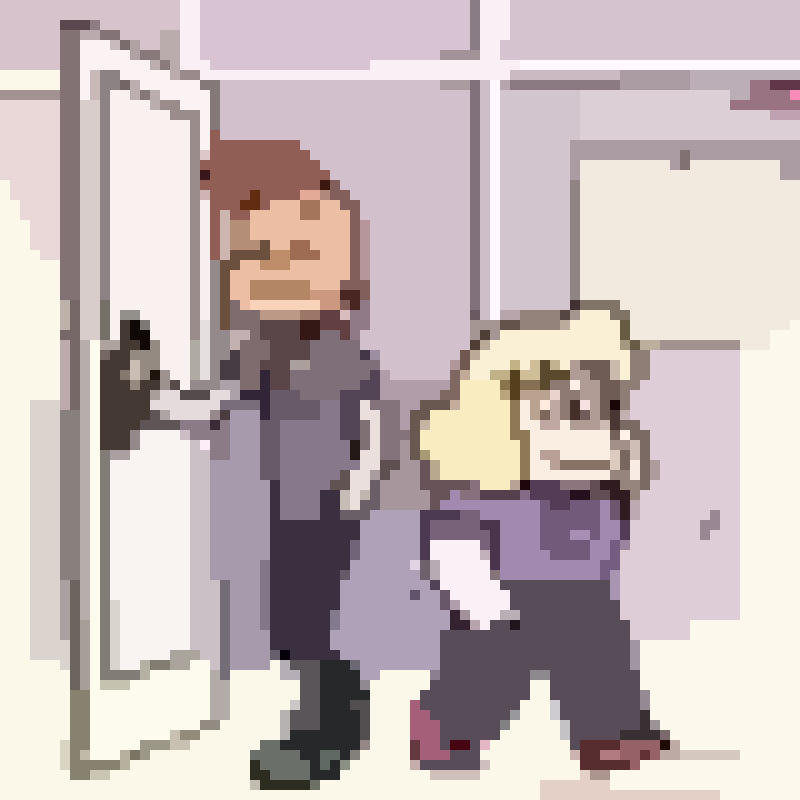
\includegraphics[width=\linewidth]{alphaResults/sadylars_large_0800.png}
\caption{$\lambda = 800$}
\end{subfigure}
\begin{subfigure}{.48\linewidth}
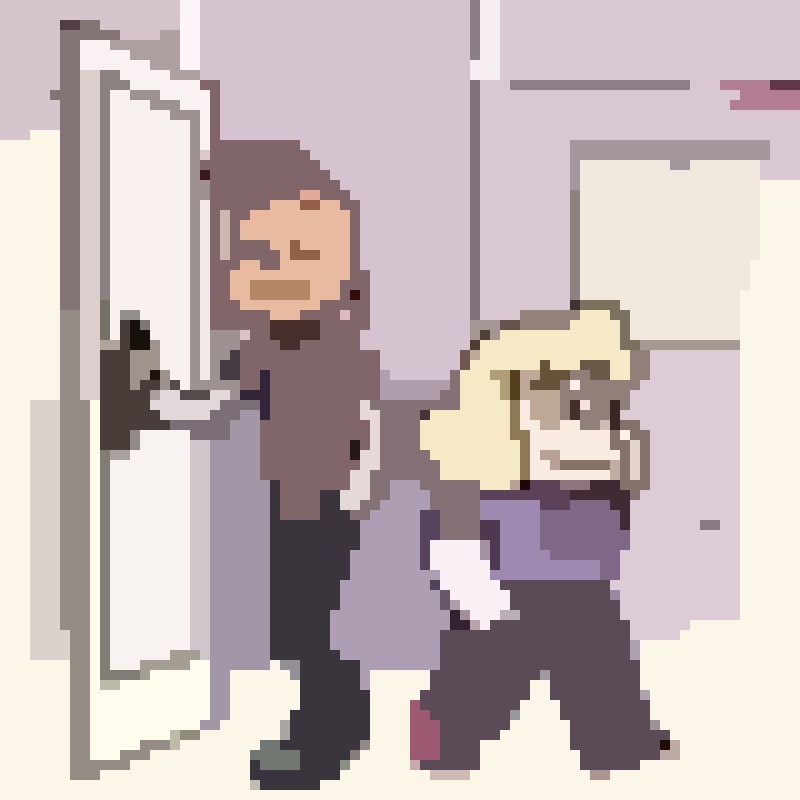
\includegraphics[width=\linewidth]{alphaResults/sadylars_large_1600.png}
\caption{$\lambda = 1600$}
\end{subfigure}
\caption{Results of $\alpha$-expansion over different values of $\lambda$, zoomed in to see results more easily. These results were generated by the grayscale transfer method.}
\label{fig:alphaResultsSadylars}
\end{figure*}

\begin{figure*}
\centering
\begin{subfigure}{.48\linewidth}
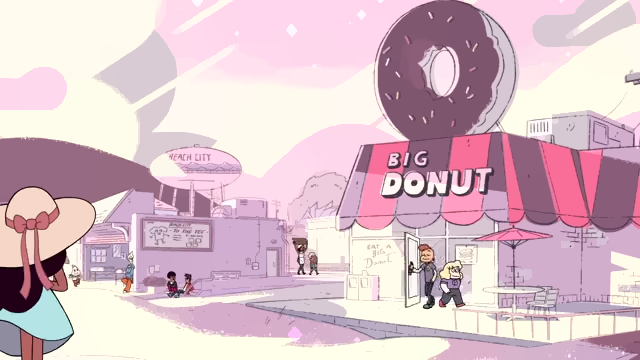
\includegraphics[width=\linewidth]{gradminResults/gradmin_1.png}
\caption{$\lambda = 0.001$}
\end{subfigure}
\begin{subfigure}{.48\linewidth}
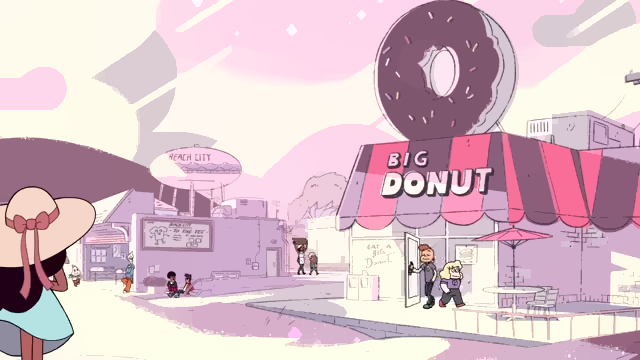
\includegraphics[width=\linewidth]{gradminResults/gradmin_2.png}
\caption{$\lambda = 0.002$}
\end{subfigure}
\begin{subfigure}{.48\linewidth}
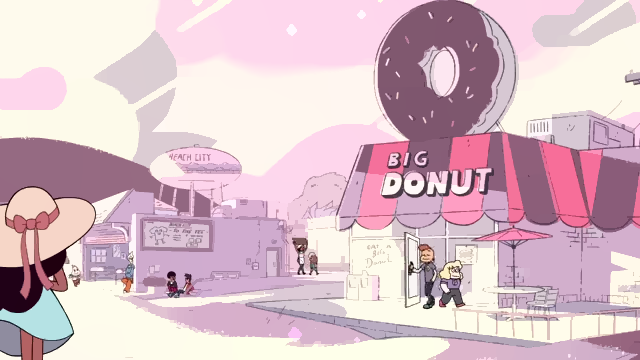
\includegraphics[width=\linewidth]{gradminResults/gradmin_4.png}
\caption{$\lambda = 0.004$}
\end{subfigure}
\begin{subfigure}{.48\linewidth}
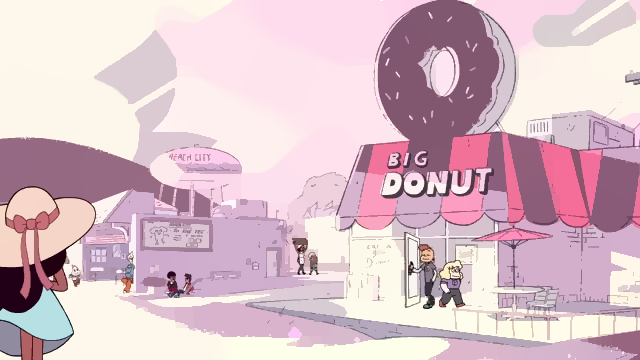
\includegraphics[width=\linewidth]{gradminResults/gradmin_8.png}
\caption{$\lambda = 0.008$}
\end{subfigure}
\begin{subfigure}{.48\linewidth}
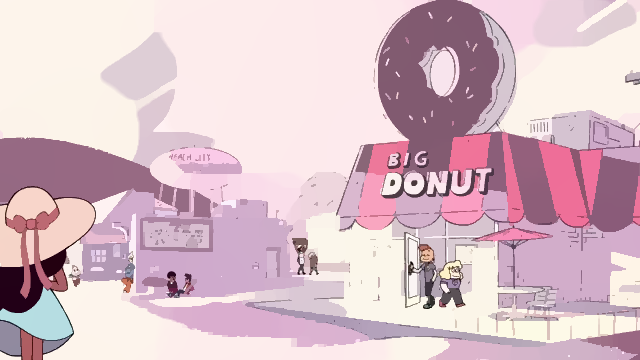
\includegraphics[width=\linewidth]{gradminResults/gradmin_16.png}
\caption{$\lambda = 0.016$}
\end{subfigure}
\begin{subfigure}{.48\linewidth}
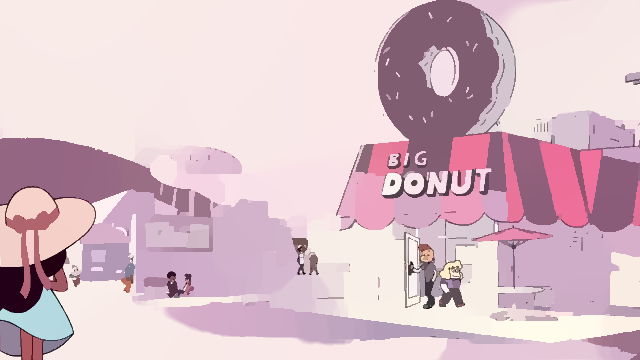
\includegraphics[width=\linewidth]{gradminResults/gradmin_32.png}
\caption{$\lambda = 0.032$}
\end{subfigure}
\caption{Results of $L_0$ gradient minimization over different values of $\lambda$.}
\label{fig:gradminResultsFull}
\end{figure*}

\begin{figure*}
\centering
\begin{subfigure}{.48\linewidth}
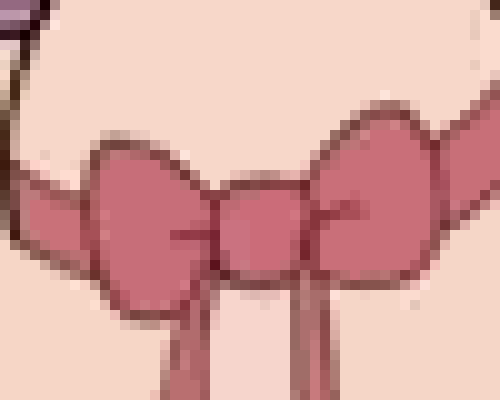
\includegraphics[width=\linewidth]{gradminResults/gradmin_bow_large_0001.png}
\caption{$\lambda = 0.001$}
\end{subfigure}
\begin{subfigure}{.48\linewidth}
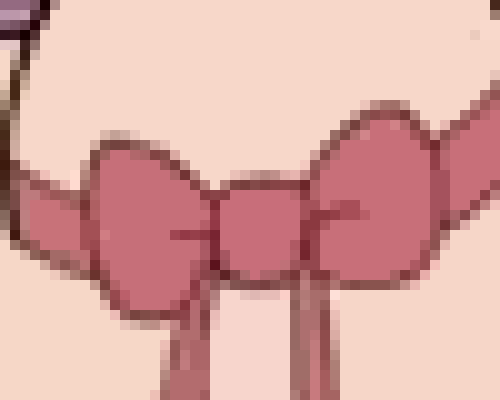
\includegraphics[width=\linewidth]{gradminResults/gradmin_bow_large_0002.png}
\caption{$\lambda = 0.002$}
\end{subfigure}
\begin{subfigure}{.48\linewidth}
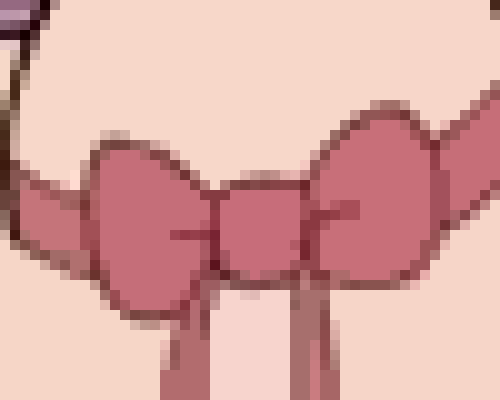
\includegraphics[width=\linewidth]{gradminResults/gradmin_bow_large_0004.png}
\caption{$\lambda = 0.004$}
\end{subfigure}
\begin{subfigure}{.48\linewidth}
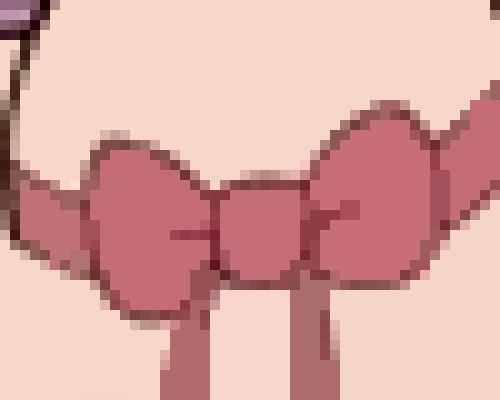
\includegraphics[width=\linewidth]{gradminResults/gradmin_bow_large_0008.png}
\caption{$\lambda = 0.008$}
\end{subfigure}
\begin{subfigure}{.48\linewidth}
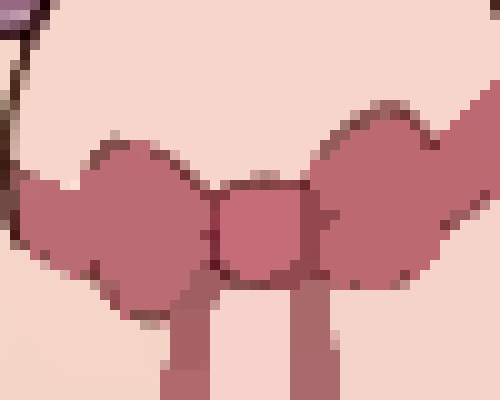
\includegraphics[width=\linewidth]{gradminResults/gradmin_bow_large_0016.png}
\caption{$\lambda = 0.016$}
\end{subfigure}
\begin{subfigure}{.48\linewidth}
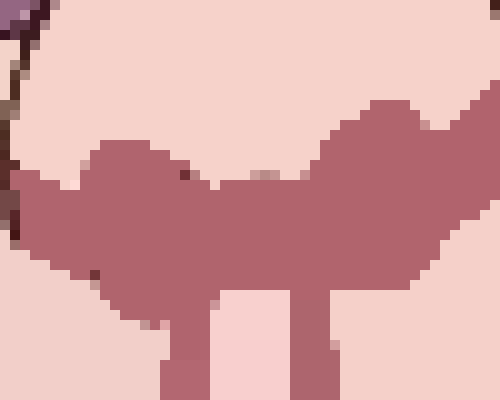
\includegraphics[width=\linewidth]{gradminResults/gradmin_bow_large_0032.png}
\caption{$\lambda = 0.032$}
\end{subfigure}
\caption{Results of $L_0$ gradient minimization over different values of $\lambda$, zoomed in to see results more easily.}
\label{fig:gradminResultsBow}
\end{figure*}

\begin{figure*}
\centering
\begin{subfigure}{.48\linewidth}
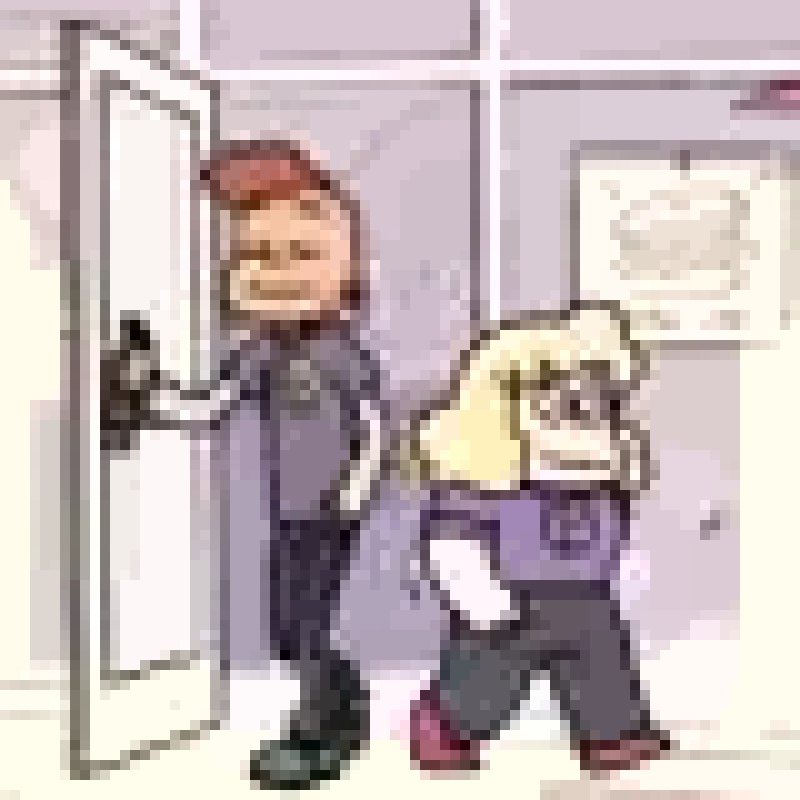
\includegraphics[width=\linewidth]{gradminResults/gradmin_sadylars_large_0001.png}
\caption{$\lambda = 0.001$}
\end{subfigure}
\begin{subfigure}{.48\linewidth}
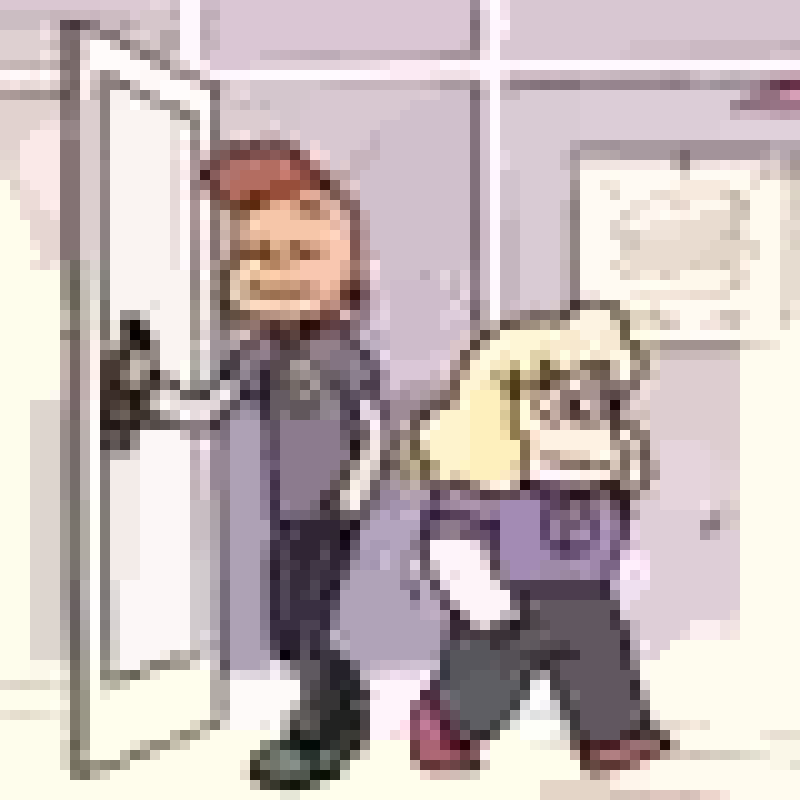
\includegraphics[width=\linewidth]{gradminResults/gradmin_sadylars_large_0002.png}
\caption{$\lambda = 0.002$}
\end{subfigure}
\begin{subfigure}{.48\linewidth}
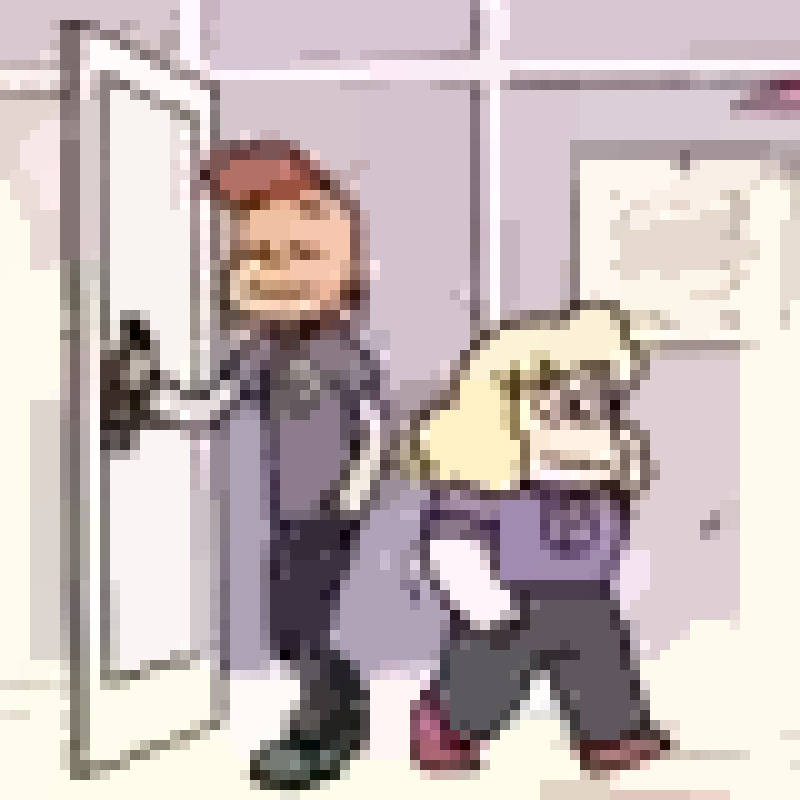
\includegraphics[width=\linewidth]{gradminResults/gradmin_sadylars_large_0004.png}
\caption{$\lambda = 0.004$}
\end{subfigure}
\begin{subfigure}{.48\linewidth}
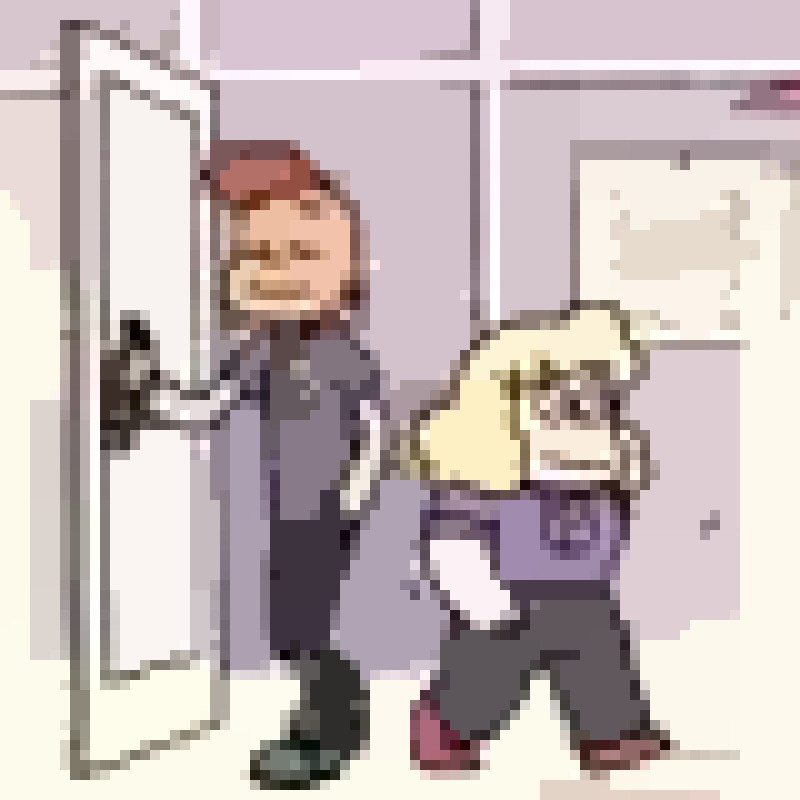
\includegraphics[width=\linewidth]{gradminResults/gradmin_sadylars_large_0008.png}
\caption{$\lambda = 0.008$}
\end{subfigure}
\begin{subfigure}{.48\linewidth}
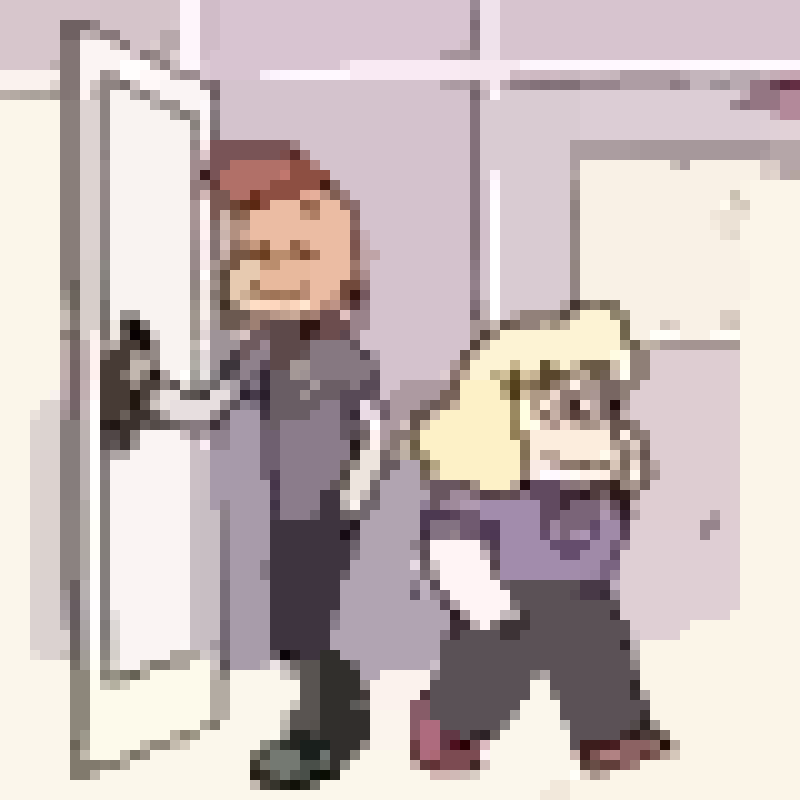
\includegraphics[width=\linewidth]{gradminResults/gradmin_sadylars_large_0016.png}
\caption{$\lambda = 0.016$}
\end{subfigure}
\begin{subfigure}{.48\linewidth}
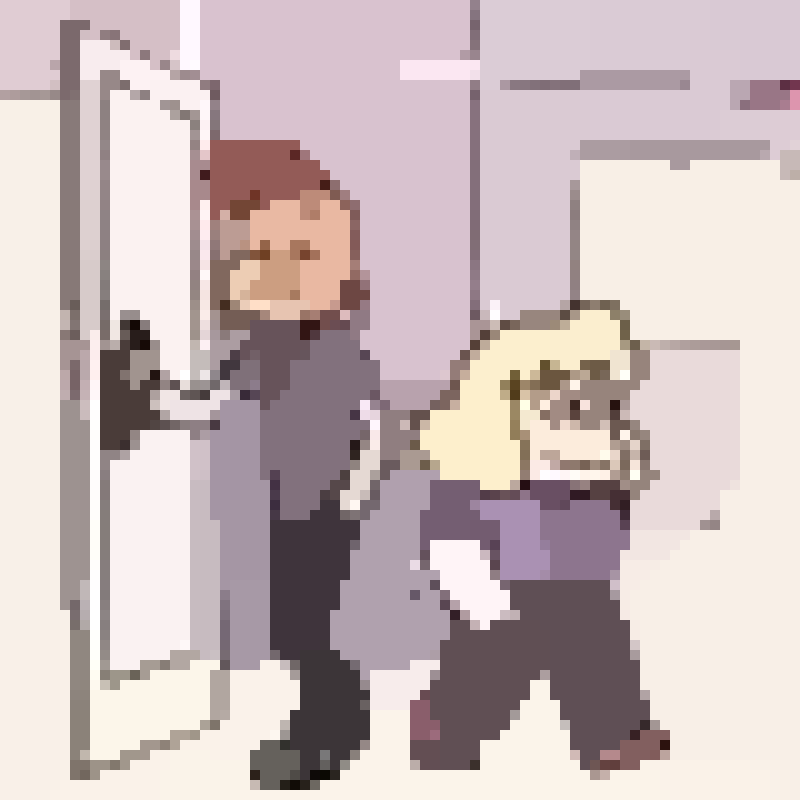
\includegraphics[width=\linewidth]{gradminResults/gradmin_sadylars_large_0032.png}
\caption{$\lambda = 0.032$}
\end{subfigure}
\caption{Results of $L_0$ gradient minimization over different values of $\lambda$, zoomed in to see results more easily.}
\label{fig:gradminResultsSadylars}
\end{figure*}

{\small
\bibliographystyle{ieee}
\bibliography{refs}
}

\end{document}